%!TEX root = main.tex
\chapter{Implementation}
\label{chap:implementation}
This chapter described the PeacefulBanana architecture, the technology we used to implement it and the functionality it provides. 

\section{Application Architecture}
As described in Section \ref{subsec:archirequire}, the application is implemented with a client-server architecture and all related requirements is described in \ref{subsec:archirequire}. Figure \ref{ClientServerGithub} shows an overview of the system design and the interaction between users, the web-server and GitHub. Each PeacefulBanana user visits the web-application through a web-browser. PeacefulBanana runs on a dedicated server and is able to serve many users at the same time. In the background the PeacefulBanana application communicates with GitHub through the GitHub API (See Section \ref{githubapi}) and synchronizes project and user-data in real time while users perform their tasks. Users connect their local PeacefulBanana account with their GitHub account in order to gain access to projects. All data collected from GitHub is stored locally on the server in a database (See section \ref{sec:database}). 
\begin{figure}[H]
    \centering
        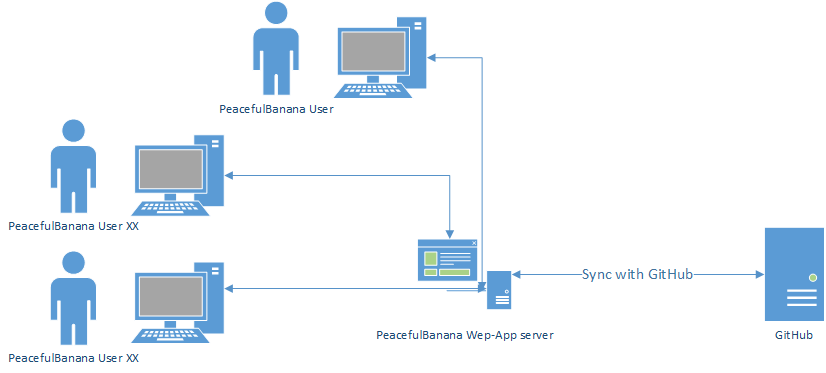
\includegraphics[width=\textwidth]{Clientservergithub}
    \caption{Overview of system design.}
    \label{ClientServerGithub}
\end{figure}

\section{Technology}
When choosing a framework for the prototype, several alternatives like Spring\footnote{\url{http://www.springsource.org/}}, WebObjects\footnote{\url{htpp://www.apple.com/webobjects/}} and Play Framework\footnote{\url{http://www.playframework.com/}} where discussed. Their architecture and our familiarity to the framework was a vital part of the selection. Based on these criteria the server was implemented with Grails a framework for web applications, it is better described in Section \ref{sec:grails}. 

\subsubsection{GitHub API}
\label{githubapi}
GitHub provides developers with the opportunity to use an API\footnote{Application programming interface} which gives them the possibility to communicate with GitHub and retrieve data directly from their database. The identified requirements concerning GitHub is described in Section \ref{sec:githubreq}.

When retrieving data from GitHub we used the provided API as described by their developer-site\footnote{\url{http://developer.github.com/v3/}}, this enabled us to control the sequence of data and when to ask for what type of data. All communication to GitHub servers are asynchronous and while therefore not introduce any performance related issues. 

The application needs to authenticate with GitHub in order to , through the use of OAUTH2 tokens. When the user first uses the tool, he will be asked to authenticate with GitHub's authentication page, asking the user to log in and authorize the PeacefulBanana tool. When this is done the tool receives a token it can use on behalf of the user to retrieve data from GitHub. The token itself is not stored, but retrieved in the background when required and bound to the users HTTP-session which expires when the user closes the browser window. This is done for safety reasons cause it would be devastating if these tokes got in the hands of the wrong people, they could for example delete the entire repository.

For gathering data from GitHub, data is transfered as JSON(JavaScript Object Notation), a lightweight data interchange language. 
 
\subsubsection{Grails}
\label{sec:grails}
The PeacefulBanana application was developed with the Grails framework. 
Grails is an open source web application framework which uses the programming language Groovy(which is built on top of the Java Virtual Machine). When Grails was developed, it's developers aimed to re-use proven technologies such as Hibernate\footnote{\url{http://www.hibernate.org/}} and Spring\footnote{\url{http://www.springsource.org/}}.  

\begin{figure}[H]
\centering
    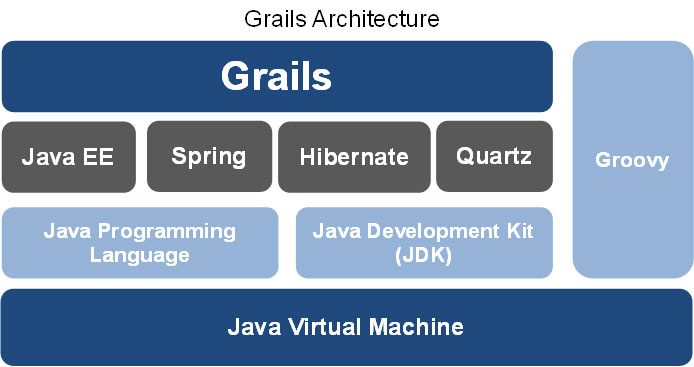
\includegraphics[width=0.8\textwidth]{Grails-Architecture}
\caption{Overview of Grails architecture \citep{grailsarchitecturediagram}}
\end{figure}

Architecturally, Grails is designed with the MVC\footnote{Model View Controller} pattern as a basis, this will expose the model\footnote{Data stored about the object.} in the view\footnote{With the restrictions on what data is viewable for the user.} and any manipulations to the model is done through a controller which controls that the data is correct input to the fields and what fields can be manipulated. An overview of the paradigm can be viewed in figure \ref{mvc-paradigm} below.

This pattern makes it easy for the developer to remain in control when creating a user interface and will ensure that the user can not manipulate fields without going through the controller\citep{reenskaug2009dci}. Using MVC increases flexibility and re-use by decoupling the user interface from the model and controller parts. The content of the view must reflect the state of the model, meaning when the model changes it notifies the view, which in turns updates itself. 
\begin{figure}[H]
    \centering
        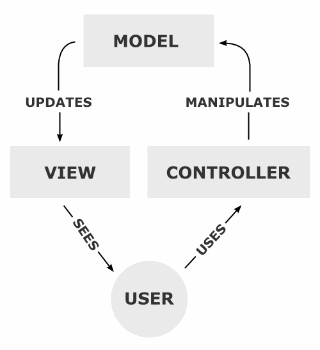
\includegraphics[width=0.7\textwidth]{MVC}
    \caption{Model-view-controller paradigm \citep{mvcmodel}}
    \label{mvc-paradigm}
\end{figure}

\subsubsection{Spring Security}
For authentication and access-control we used the \emph{Spring Security} framework, which is a part of Spring. Spring Security allowed us to create user accounts and connect these within the application. Functionality like changing password, requesting new password when forgotten are examples of what Spring Security provides. Requirements related to authentication and security, is described under \emph{General Requirements} in Section \ref{sec:genreq}. Requirements related to user accounts, and linking users to teams is described in Section \ref{sec:teamreq}.

\subsubsection{jQuery}
jQuery was initially released under the MIT license in 2006 to make it easier to select DOM\footnote{Document-Object-Model} objects and create powerful dynamic web pages and applications.

JQuery provided our application with a way to change objects in real-time without refreshing the whole page, using AJAX\footnote{Asynchronous JavaScript and XML - AJAX is a way to change the contents DOM objects asynchronous from JavaScript.}.

\subsubsection{AwesomeCloud}
Awesome cloud is a plugin for jQuery for creating a tag cloud. It retrieves data from DOM-objects and renders them as a cloud, where the font-size increases with the occurrence of tags. The tag cloud is then drawn on the HTML5 canvas. We used this to implement our individual and team-wide tag-clouds (See Section \ref{sec:corefunctionality}). 

\subsection{Server and Database}
\label{sec:database}
The PeacefulBanana application was deployed on a Ubuntu server running Apache Tomcat v7. Server related requirements is described in Section \ref{sec:serverreq}.  
During development we ran the application on a H2\footnote{\url{http://www.h2database.com/}} in-memory database. However the need for persistent storage arose, so we migrated to a MySQL database in order for the data to stay unchanged when we had to roll out updates to the tool. This choice was essential for the tool to function as described in the requirements, but the H2 database was more convenient and faster to debug during development.
\subsubsection{MySQL}
MySQL\footnote{MySQL: \url{http://www.mysql.com/}} is the world's largest open source relational database management system and can be used for a variety of applications. It is most commonly used with Web applications and works very well with dynamic web-pages, meaning that the content of each page is generated based on data loaded from a database as the page loads.

\subsubsection{Database description}
The PeacefulBanana GitHub specific domain-classes can be seen in Figure \ref{GithubDomainClasses}, and shows the relationship between the different data retrieved through the GitHub API. 
All \emph{User specific} domain-classes can be seen in Figure \ref{UsersDomainClasses}.

A detailed walkthrough with data type categorization and description can be seen in Appendix \ref{app:database}
\begin{figure}[H]
    \centering
        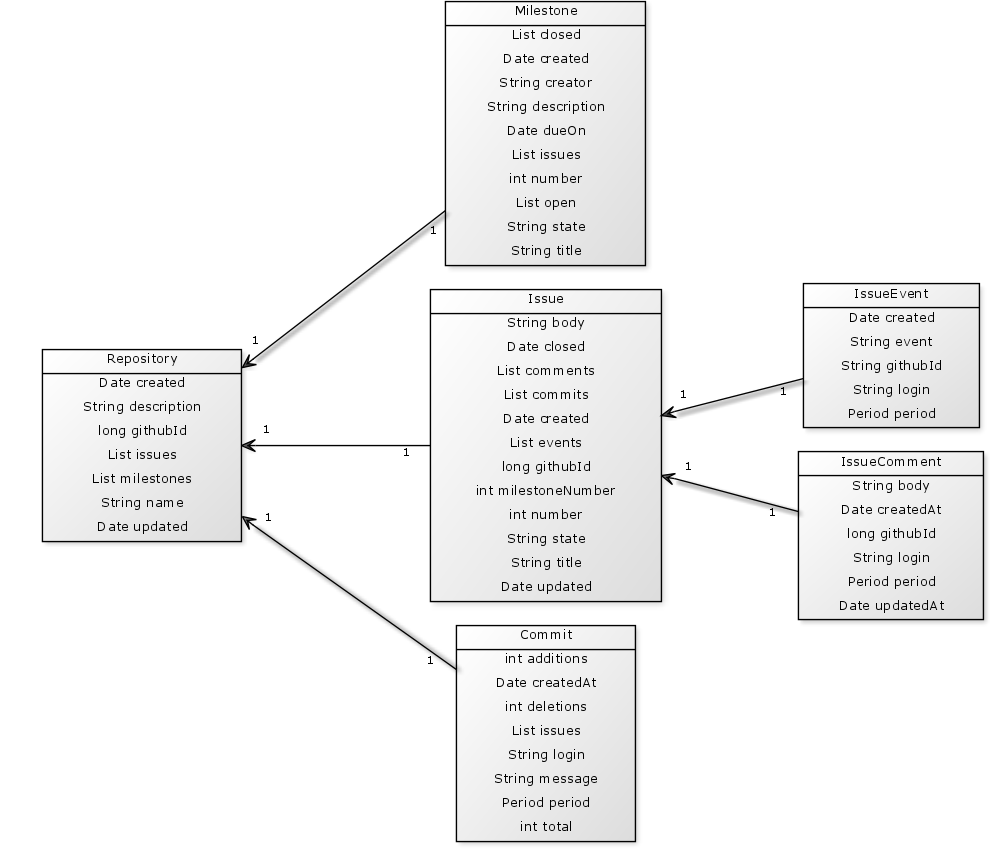
\includegraphics[width=\textwidth]{GithubDomainClasses}
    \caption{GitHub domain classes}
    \label{GithubDomainClasses}
\end{figure}
\begin{figure}[H]
    \centering
        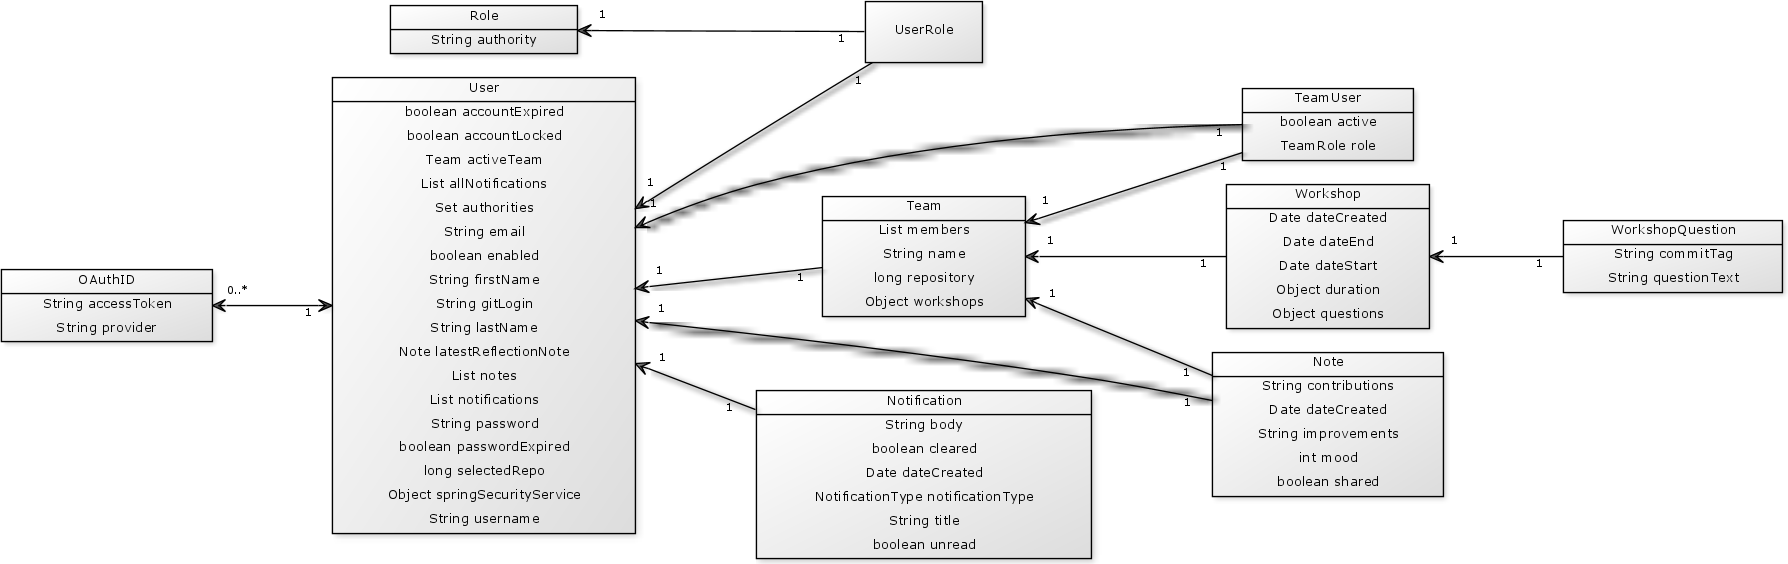
\includegraphics[width=\textwidth]{UsersDomainClasses}
    \caption{User domain classes}
    \label{UsersDomainClasses}
\end{figure}
